\documentclass{ximera}

%\addPrintStyle{..}

\begin{document}
	\author{Bart Lambregs}
	\xmtitle{Denkvragen}{}
    \xmsource\xmuitleg



\begin{exercise}
	Kan een voorwerp bewegen zonder dat er een kracht op werkt?% Leg uit.
\end{exercise}

\begin{exercise}
	Waarom is een met boomstammen geladen vrachtwagen voor de bestuurder zo gevaarlijk, als hij bruusk moet remmen, of bij een botsing betrokken raakt?

	\begin{oplossing}
		De boomstammen willen volgens de eerste wet van Newton tijdens het remmen hun beweging voortzetten.
	\end{oplossing}
\end{exercise}

\begin{exercise}
	Hoe komt het dat een vrachtwagen binnen een veel kortere afstand kan stoppen dan een trein die dezelfde snelheid heeft?
\end{exercise}

\begin{exercise}
	Wat word je gewaar als je met een wapen een kogel afvuurt? Waarom druk je best de kolf stevig tegen de schouder aan?
\end{exercise}

\begin{exercise}
	Hoe komt het dat je gemakkelijk vaststelt dat de aarde een kracht uitoefent op een appel, maar dat je niets merkt van de kracht door de appel op de aarde uitgeoefend?
\end{exercise}
%Hoe komt het dat het de appel is die naar de aarde valt en niet andersom, terwijl de derde wet van Newton zegt dat beide lichamen een even grote maar tegengestelde kracht op elkaar uitoefenen?

\begin{exercise}
	Wat gebeurt er met een roeiboot als men snel van de voor- naar de achterkant loopt?
\end{exercise}

\begin{exercise}
	Op een bierglas ligt een plastic plaat met daarop een appel. Als Els de plaat snel wegtrekt valt de appel in het glas. Bij Lien die de plaat langzaam wegtrekt, niet. Verklaar het verschil tussen beide verschijnselen.

	\begin{oplossing}
		Als je de plaat snel wegtrekt, is de wrijvingskracht te kortstondig aanwezig om de appel een noemenswaardige versnelling te geven. Trek je traag, dan is de versnelling misschien klein maar is ze lang genoeg aanwezig om de appel een voldoende grote snelheid te geven.
	\end{oplossing}
\end{exercise}

\begin{exercise}
	Wat klopt er fysisch niet aan wat er gebeurt in de cartoon?% Licht toe.

	\begin{image}
		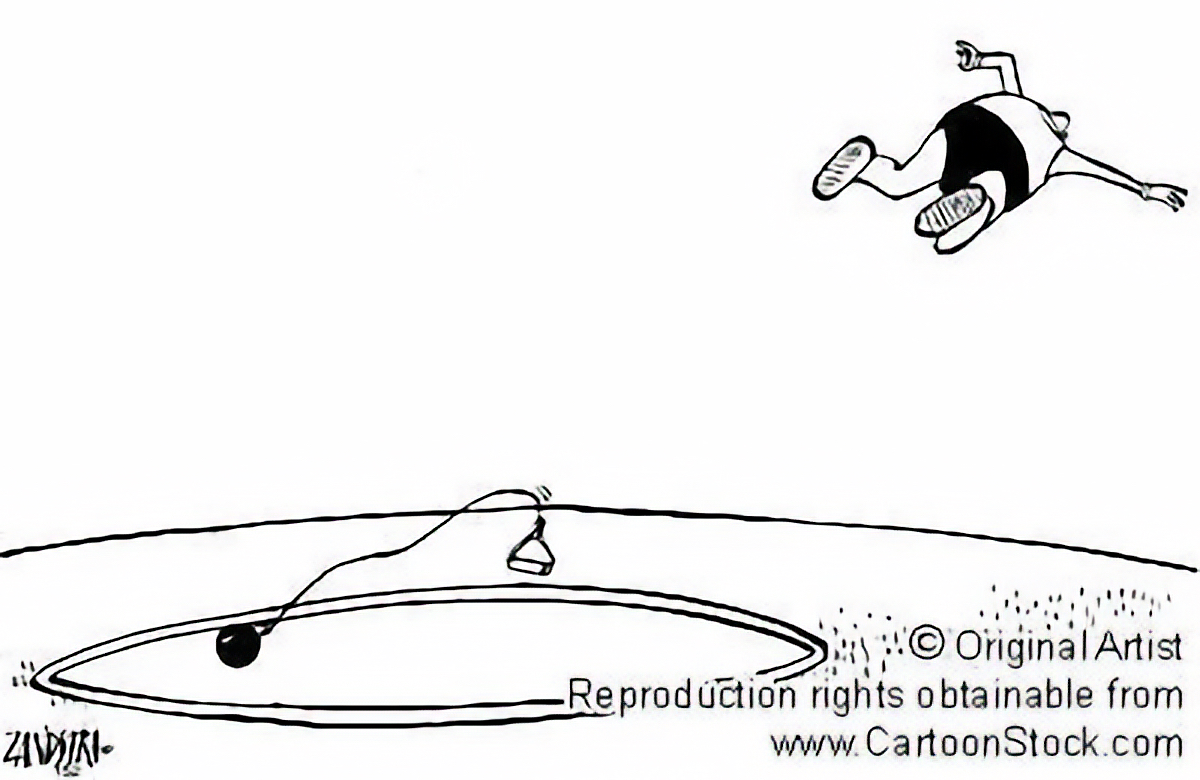
\includegraphics[width=.4\textwidth]{jza0018l}
	\end{image}
\end{exercise}

\begin{exercise}
	Waarom valt in het luchtledige een massa van \SI{2}{kg} niet twee keer zo snel als een massa van \SI{1}{kg}?
	%De zwaartekracht op een steen van $2\rm\,kg$ is tweemaal zo groot als de zwaartekracht op een steen van $1\rm\,kg$, en toch vallen beide stenen even snel. Hoe komt dat?

	\begin{oplossing}
		In het vacu\"um werkt op een vrije massa enkel de zwaartekracht in. Dat is dan ook de resulterende kracht op de massa. Die kracht is inderdaad twee keer zo groot voor een twee keer zo grote massa, maar een twee keer zo grote massa verzet zich ook twee keer zo hard tegen het het veranderen van beweging; de traagheid is twee keer zo groot. Het resultaat is dat elk object met dezelfde versnelling naar de aarde valt.

		Die hierboven eerder kwalitatieve redenering is kwantitatief uit te leggen met de tweede wet van Newton, $\vec{F}=m\vec{a}$:
		\begin{equation*}
			F_z=ma
		\end{equation*}
		Met de formule $F_z=mg$ voor de zwaartekracht vinden we
		\begin{equation*}
			mg=ma
		\end{equation*}
		Zodat, na de massa's te hebben geschrapt
		\begin{equation*}
			a=g
		\end{equation*}
		De massa van het object heeft m.a.w. geen invloed op de versnelling waarmee het valt. Die versnelling is constant en in waarde gelijk aan de waarde van de veldsterkte. Omdat ook de eenheden overeenkomen (uit de tweede wet van Newton volgt dat \SI{}{N}=\SI{}{kg\cdot m/s^2}) wordt het symbool $g$ voor zowel de veldsterkte als de valversnelling gebruikt. Bij ons heeft die de waarde \SI{9,81}{m/s^2}.
	\end{oplossing}
\end{exercise}




	
\end{document}